We have seen that replica selection flexibilities can render embeddings computationally hard.
We will now provide a more detailed look at this hardness result
and explore the minimal requirements for rendering replica selection hard.
In particular, we will show that already two replicas for each chunk type are sufficient to
introduce intractability.

Namely, we provide the NP-hardness results for two restricted variants of Virtual Cluster Embedding (Sections~\ref{ap:tworep-ma} and \ref{ap:tworep-ni}).
We augment the $\RS$ variant of $\VCEMB$ problem in the following way: by $\RS(k)$ we denote the problem where each chunk has the redundancy factor at most $k$.
In Section~\ref{ap:tworep-ma} we provide the hardness result for $\RS(2)+\MA+\FP$, and in Section~\ref{ap:tworep-ni} we provide the hardness result for $\RS(2)+\FP+\CC+\BW$.

Both problems are reduced from the problem $\TDPM$ (see Section~\ref{sec:3dm_intro} with no further restrictions.
The constructions are based upon the reduction of $\TDPM$ to $\FP+\RS+\MA$ (see Section~\ref{ssec:fprsma}) and the reduction of $\TDPM$ to $\FP+\RS+\CC$ (see Section~\ref{ssec:fprscc}).
However, in contrast to Section~\ref{ssec:fprscc}, in two replica variant without multiple assignment, we added the bandwidth constraints.
It is currently unknown to the authors of this very paper, whether the hardness result holds without bandwidth constraints (namely, whether the problem $\RS(2)+\FP+\CC$ is NP-hard).
The necessity for bandwidth constraints arises as to deal with restricted factor of replication, we need to introduce gadgets in the tree that makes the tree asymmetric.
Introducing bandwidth constraints allows to control the number of nodes spawning in certain parts of the tree.

\subsection{Two Replicas without Bandwidth Constraints}\label{ap:tworep-ma}

We now show that the 2-replica selection problem is even NP-hard
without capacity constraints.  In particular, we consider the problem
variant~$\RS(2)+\MA(4)+\FP$ with at most two replicas of each chunk type and assignment factor
four. There are no capacity constraints on links.

Our construction consists of two major modifications to hardness result without replication factor restrictions (for that result, refer to Section~\ref{ssec:fprsma}).

\textbf{Unique chunks on the comb.} First, we provide the tools for restricting the placement of nodes in certain parts of the tree.
In Section~\ref{ssec:fprsma}, due to symmetric structure of the tree, the carefully crafted threshold value allowed us to proof that e.g. no Triple Gadget ever had two or more nodes placed in it.
We still use the threshold value as the placement mechanism, but in this section, due to asymmetrical tree construction, we cope it with the concept of unique chunks on the comb (by the \emph{comb} we denote the balanced tree, where all non-root vertices has at most one child).

For the introduction to the concept of unique chunks, see the following example.
Suppose that within one $\VCEMB$ construction, we would like to encode not one $\TDPM$ instance, but two $\TDPM$ instances: $M_1$ and $M_2$, with disjoint universe and distinct number of triples to be chosen: $n_1$ and $n_2$.
We perform the following modifications to encoding provided in Section~\ref{ssec:fprsma}.
The multi-assignment factor grows by $1$, that is the instance we construct is the $\RS+\MA(4)+\FP$ instance.
We construct two subtrees $T_1$ and $T_2$, that correspond to resp. $M_1$ and $M_2$; we construct two two-edge-level combs $C_1$ and $C_2$, with number of leaves $n_1$, resp. $n_2$.
We attach $M_1$ and $C_1$ (resp. $M_2$ and $C_2$) to the common root and we name the resulting subtree the $P_1$, resp. $P_2$.
Next, we attach $P_1$ and $P_2$ to the common root.
In the end, the height of the tree grew by $2$.
Finally, we populate both combs with unique chunks, and we set the number of to-be-placed nodes to $n_1+n_2$.
We modify the threshold to be sum of the threshold for constructions for $M_1$ and $M_2$ plus $4\cdot (n_1 + n_2)$.
The last substrate of the threshold value corresponds to transportation of fourth chunk processed by each machine for the distance of four.

To see why the example indeed can solve two instances of $\TDPM$, we need the following observations.
First, we claim that no node is ever placed in a comb.
To prove this fact, we use the property of the comb that the leaves are highly separated, and the fact that each machine has to process $4$ chunks.
Next, we claim that the number of nodes spawned in $P_1$ (resp. $P_2$) is $n_1$ (resp. $n_2$).
To see this, consider any imbalance of number of spawned nodes; notice that some chunks in the underpopulated comb are processed outside of its $P_i$ subtree, resulting in the solution that exceeds the threshold.

\textbf{Families of chunk types.} The second tool that we introduce allows us to express the redundancy of chunks without actually replicating chunks more than two-fold.
For simplicity of introduction, we consider the scenario with multi-assignment factor of $1$.
For each chunk type $c$ with redundancy, we count the number of occurrences of replicas of such chunk in the tree, and name it $r_c$.
We replace the chunk type $c$ with $r$ chunk types, which we call the family $F_c$ of that chunk type.
For each occarrence of replica of $c$, we replace it with replica of any chunk type from the family (without repetitions).
To this point, the redundancy factor was reduced from $r_c$ to $1$.
Now, we construct the gadget $G_c$ for chunk type $c$, which consists of $r_c$ leaves, each hosting the second replica of each chunk type from family $F_c$.
We use the technique of unique chunks on the comb to constraint the number of nodes in $G_c$ to be exactly $r_c - 1$.
We provide necessary additional $r_c-1$ nodes to be placed.
Hence, exactly $1$ node is placed on chunk type of family $F_c$ outside the gadget $G_c$, and exactly $r_c-1$ nodes cover remaining $r_c-1$ chunk types inside gadget $G_c$.
All chunk types are processed, the replication factor was reduced to $2$, and the size of construction grew polynomially.

\textbf{Introduction to the reduction.} As we already stated, we modify the construction from Section~\ref{ssec:fprsma}.
As the way to deal with replication, we use the families of chunk types, which uses the unique chunks on the comb.
We extend the construction of a gadget for chunk type with redundancy, by incorporating the fact that the multi-assignment factor is $4$.
For the construction to remain correct with such multi-assignment factor, we introduce further chunks types with one chunk replica to place in the chunk gadget and use the excessive $3$ data processing capacities.

\textbf{Construction.}
For arbitrary instance~$I_{\TDPM}$ of~$\TDM$ we construct a~$\RS(2)+\MA(4)+\FP$ instance~$I_{\VCEMB}$ the way described in the remainder of this section.
Let $n = |X|\cup|Y|\cup|Z|$.
By $T$ we denote the set of all triples of $I_{\TDPM}$.
To access the elements of a triple $\tau \in T$, we introduce the following notation: $\tau = \langle e_X(\tau), e_Y(\tau), e_Z(\tau) \rangle$.
For each $e\in X\cup Y\cup Z$, by $T_e$ we denote the set of all triples that contain element $e$.
Let $\deg(e) = |T_e|$, and note that $\sum_e \deg(e) = 3\cdot |T|$.
Finally, let $t = |T|$.

We proceed with the construction as follows.

\paragraph{Chunk types and replicas}

We construct three types of chunks.
The first type corresponds to elements of the universe (that is, $X\cup Y\cup Z$).
The construction of such chunk types is similar to construction of chunk types in Section\ref{ssec:fprsma}, but to take into consideration the restricted replication factor, we construct the familiy of chunk types (as described in the introduction to this section).
Namely, for each element of universe $e$, we construct as many chunk types as there are occurences of $e$ in triples of $I_{\TDPM}$.
Each such chunk type has exactly two replicas.

The other two types are chunk types with one replica only, therefore called \emph{unique}.
We construct two types of unique chunks, distinguished by a different role in the construction.
For unique chunks we simply co-notate the chunk type with chunk replica.

Formally, the construction of chunk types and replicas unfolds as follows:
\begin{enumerate}
  \item For each triple $\tau \in T$, we construct $3$ chunk types, with two replicas each.
  We construct different chunk types for each triple $\tau$, which contain element $e$ (in total $\deg(e)$ chunk types).
  We refer to those replicas by $ch_1(e, \tau)$ and $ch_2(e, \tau)$.
  In total we construct $2\cdot \deg(e)$ chunk replicas.
  \item We construct~$n$ additional chunk types named
  ~$u_1, \ldots, u_n$ with one replica each.
  \item For each element~$e\in X\cup Y\cup Z$,
  we construct additional~$3\cdot(\deg(e) - 1)$ chunks, with one replica each.
  We call this set~$\UniqueE$.
\end{enumerate}

\paragraph{Tree}

We construct the tree that has the following structure (see Figure~\ref{fig:red-ma}):

\begin{figure}[t]
  \centering
  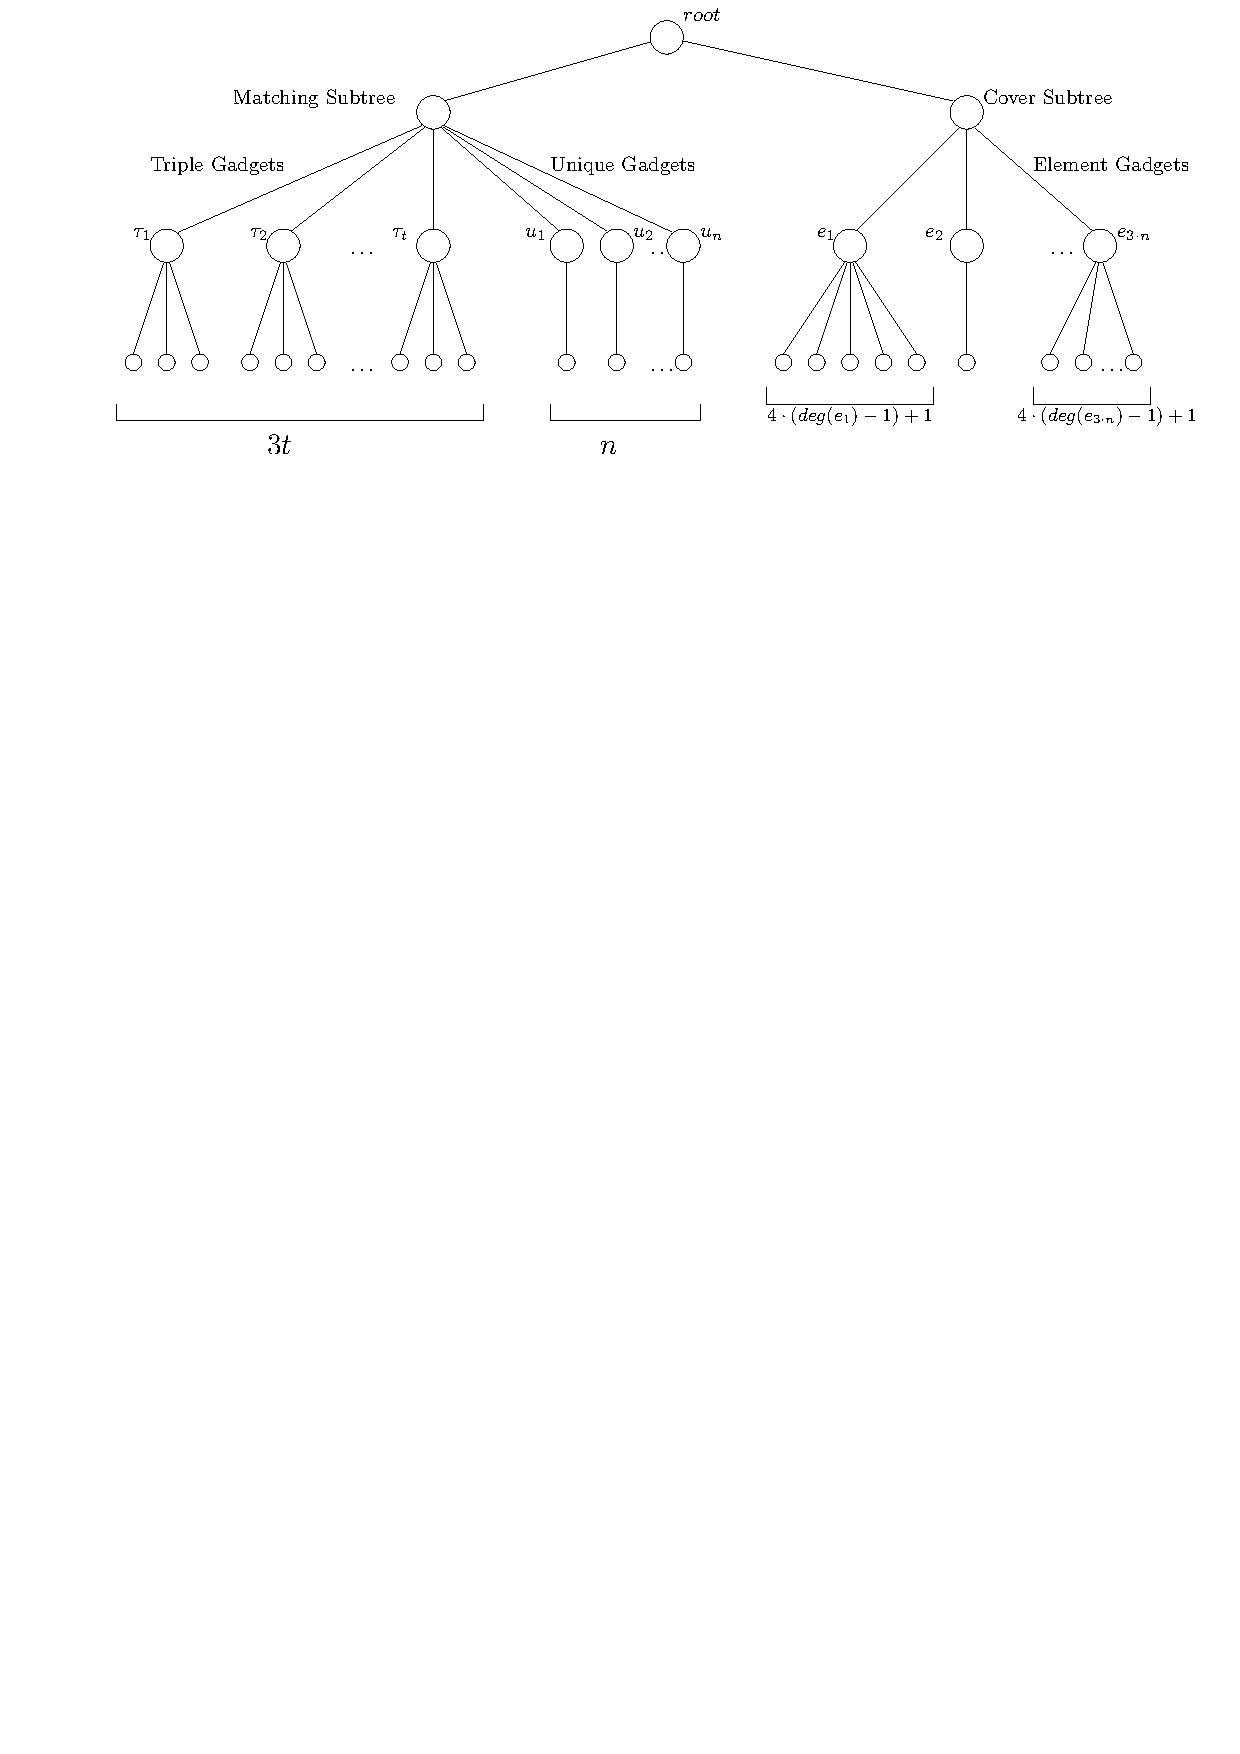
\includegraphics[width=0.99\columnwidth]{reduction/overview.pdf}
  \label{fig:red-ma}
  \vspace{-1em}
  \caption{Overview of the substrate network}
  \vspace{-1em}
\end{figure}


\begin{enumerate}
  \item The physical network consists of two subtrees connected to the
  root: A {\MatchSubtree} and a {\CoverSubtree}. The
  {\MatchSubtree} consists of $t$ {\TripleGadgets}, one per each triple $\tau\in T$ and $n$
  {\UnqGadgets}. The {\CoverSubtree} consist of~$3\cdot n$ {\ElGadgets}, one for each element $e\in X\cup Y\cup Z$ \maciek{TODO: wrong in picture}.
  \item {\TripleGadget} consists of four vertices: three leaves and the root of the gadget.
  \item {\UnqGadget} consists of two vertices: the leaf and the root of the gadget.
  We construct the root node of the gadget not only to keep the tree balanced, but also to keep leaves of
  {\UnqGadgets} far from leaves of other \UnqGadgets. Note that \UnqGadgets{} form a comb.
  \item {\ElGadget} of element $e$ has a structure that depends on the number of triples that cover $e$. The {\ElGadget} consists of the
  root, and~$4\cdot(\deg(e)-1)+1$ leaves.
\end{enumerate}

\paragraph{Chunk Placement}
The chunks are placed as follows:
\begin{enumerate}
  \item \emph{Chunks in the Matching Subtree:} In {\TripleGadget} of triple $\tau$ we put
  three replicas:
 ~$ch_1(e_X(\tau), \tau), ch_1(e_Y(\tau), \tau), ch_1(e_Z(\tau), \tau)$, one per each leaf.
  \item \emph{Chunks in the Unique Subtree:} We place replicas
 ~$u_1,\ldots, u_n$ at the leaves of \UnqGadgets.
 \item \emph{Chunks in Element Gadgets:} Consider the \ElGadget{} for the element $e \in X\cup Y\cup Z$.
 We place two types of replicas in the leaves of the gadget.
 We put replicas $ch_2(\tau, e)$ for each $\tau \in T_e$.
 Additionally, we place all the replicas from set $\UniqueE$.
 In total, we place $4\cdot (\deg(e) - 1) + 1$ replicas, one per each leaf of the gadget.
\end{enumerate}

\paragraph{Other properties of the instance}
\begin{enumerate}
  \item \emph{Multiple assignment:} We set the multi-assignment factor to $4$.
  \item \emph{Number of nodes:} We allow to spawn
 %~$\numNodes = n + \sum_{e}(\deg(e)-1)$ nodes.
 ~$\numNodes = n + \sum_{e}(\deg(e)-1) = 3\cdot t - 2\cdot n$ nodes.
 \item \emph{Threshold:} We set the following threshold:
 %~$\Thr = 8\cdot n + 6\cdot\sum_{e}(\deg(e)-1)$
 ~$\Thr = 18\cdot t + 5\cdot n$.
 This value corresponds to the cost of solution, where $n$ nodes process $4$ chunks that are in distance: $0, 2, 2$ and $4$ to the node, and remaining $|V|-n$ nodes process $4$ chunks that are in distance: $0, 2, 2$ and $2$ to the node.
\end{enumerate}

\textbf{The reduction.}

Before we start the reduction, let us introduce two functions that will help us show that certain node placements are infeasible, as their cost exceeds the threshold.
For each $u \in \{ 0, \ldots, n \}$ let us define~$\CostEstimOne(u) = 8\cdot n + 6\cdot t - 4\cdot u$.
We use the function $\CostEstimOne(u)$ in Lemma~\ref{th:no-unique} to show that no node spawned in the \UnqGadget{}: the $\CostEstimOne(u)$ is the lower-bound on the total cost of the solution, assumming that $u$ nodes spawned in \UnqGadgets{}.
By Lemma~\ref{lem:cost-estims}, for non-zero $u$ the cost lower-bound already exceeds the threshold.
Note that $\CostEstimOne(0) = \Thr$.

\begin{lemma}
  Every solution with $u$ nodes spawned in \UnqGadgets{} has cost at least $\CostEstimOne(u)$.
\end{lemma}
\begin{proof}
  The proof follows from the properties of the tree.
  Each node $v\in V$ spawned in \ElGadget{} incurrs the transportation cost at least $6$, as $v$ is collocated with at most one replica, and remaining $3$ replicas (remember that multi-assignment factor is $4$) are transported for at least $2$ hops.
  Each node $v\in V$ spawned in \TripleGadget{} incurrs the transportation cost at least $8$, as $v$ is collocated with at most one replica, at most two replicas that are assigned to $v$ are in the same \TripleGadget{}, hence those are transported over $2$ hops, and the last remaining replica is transported over at least $4$ hops.
  Each node $v\in V$ spawned in \UnqGadget{} incurrs the transportation cost at least $12$, as $v$ is collocated with at most one replica, and remaining $3$ replicas are transported over at least $4$ hops.
  At most $\sum_e(\deg(e)-1)=t-3\cdot n$ nodes can spawn in \ElGadget{}.\maciek{Wrong!}
  For the remaining $n$ nodes, by lemma assumption $u$ nodes spawn in \UnqGadgets{}, hence at least $n-u$ nodes spawn in \TripleGadgets{}.
  Let $c_E$ and $c_T$ be the number of nodes spawned in \ElGadget{} and \TripleGadget, respectively.
  The lower-bound on the total cost is then $6\cdot c_E + 8\cdot c_T + 12\cdot u$.
  As $c_T \leq t-3\cdot n$ and $c_E+c_T+u=\numNodes$, the total cost is at least $6\cdot (t-3\cdot n) + 8\cdot (n-u) + 12\cdot u = \CostEstimOne(u)$.\maciek{Wrong!}
\end{proof}

We define $\ldots$ and $\CostEstimTwo(u) = \ldots$.

We use the function $\CostEstimTwo$ in Lemma~\ref{th:np-balance} to show that exactly $n$ nodes spawned in the Matching Subtree. \maciek{After fixing the proof np-balance, write what $u$ corresponds to}

\begin{lemma}
  For each $u \in \{ 1, \ldots, t-1 \}$ we have that $\CostEstimOne(u) > \Thr$ and
  $\CostEstimTwo(u) > \Thr$.
  \label{lem:cost-estims}
\end{lemma}

\begin{proof}
  We have that $\CostEstimOne(u+1) \geq \CostEstimOne(u)$ and $\CostEstimTwo(u+1) \geq \CostEstimTwo(u)$ , for
 ~$1\leq u \leq t-1$. It is easy to verify that $\CostEstimOne(1) > \Thr$ and $\CostEstimTwo(1) > \Thr$.
\end{proof}

\begin{lemma}
  Take any feasible solution~$\Solution$ to the instance~$I$ of
 ~$\RS(2)+\MA(4)+\FP$ (as constructed above). If the cost of
 ~$\Solution$ is at most~$\Thr$, then no node is spawned in the Unique
  Subtree.
  \label{th:no-unique}
\end{lemma}

\begin{proof}
  For the sake of contradiction, let us assume a feasible solution
 ~$\Solution$ with at least one node spawned in {\UnqSubtree}. We show
  that in this case, the cost of solution~$\Solution$ is greater than
 ~$\Thr$. Let $\ell$ be the number of nodes spawned in the {\UnqSubtree}. We know
  that~$1 \leq \ell \leq |T|$.  In~$\Solution$ we have exactly
 ~$4 \cdot \numNodes$ chunk transportations, incurring cost
 ~$0, 2, 4$ or~$6$ (the tree has an edge-height of~$3$). At most
 ~$\numNodes$ transportations are of cost~$0$. Note that the leaves of the
  {\UnqSubtree} are separated from other leaves of the tree by at
  least~$4$ edges.  The cost of chunk transportation to nodes
spawned in the Unique Subtree is at least~$12$. The chunks in
  {\UnqSubtree} are unique, therefore the solution transports~$|T| - \ell$
  chunks to nodes outside the \UnqSubtree, incurring cost~$4$ for each
  chunk.
  Therefore $\CostSol \geq \CostEstimOne(\ell)$, and by Lemma \ref{lem:cost-estims}
  we conclude that $\CostSol > \Thr$.
\end{proof}



\begin{lemma}
  Given any feasible solution~$\Solution$ to a given instance~$I$ of
 ~$\RS(2)+\MA(4)+\FP$ (as constructed above). If the cost of
 ~$\Solution$ is at most~$\Thr$, then exactly~$n$ nodes are spawned in the
  \MatchSubtree.
  \label{th:np-balance}
\end{lemma}
\begin{proof}
    \maciek{This proof requires revision}
  Let~$\ell$ be the number of nodes spawned in
  {\MatchSubtree}.  Let us assume the contrary, namely that
 ~$\ell \neq n$.  First, we use
  Theorem~\ref{th:no-unique} to restrict the placement of nodes in
  \UnqSubtree. Then we consider two cases:
  \begin{enumerate}
    
    \item~\textbf{Case $\ell \leq n$:} There are at least
   ~$u := 4 \cdot (n-\ell)$ chunks in the {\MatchSubtree} that are not
    processed in the {\MatchSubtree}, each incurring transportation
    cost of~$6$.
     From the structure of the substrate network and placement of
    chunks we know that~$\CostSol \geq \CostEstimTwo(\ell)$, and by Lemma \ref{lem:cost-estims}
  we conclude that $\CostSol > \Thr$.
.

    \item \textbf{Case $\ell>n$:} We use the fact that there are not enough nodes in
    {\CoverSubtree}, and we need to transport over~$6$ hops at least 3
    unique chunks for each node missing from {\CoverSubtree}.
  \end{enumerate}
\end{proof}
\maciek{TODO: rewrite end}

\begin{theorem}
 ~$\RS(2)+\MA+\FP$ is NP-hard.
\end{theorem}

\begin{proof}
  
  Let's take an instance~$I$ of~$\TDPM$ and construct an instance~$I'$
  of~$\RS(2)+\MA+\FP$ in the way described in the construction section.  We show that~$I'$
  has a solution of cost~$\leq \Thr$ if and only if~$I \in \TDPM$ (there
  exists a perfect 3D matching).

  ($\Leftarrow$) Let's take any feasible solution~$\Sol$ to~$I$. We
  construct a solution~$\Sol'$ to~$I'$ in the following way:
  \begin{enumerate}
    \item We place~$n$ nodes in~$n$ {\TripleGadgets} (one per gadget)
    that correspond to triples in~$\Sol$. We match each such node
    to chunks in the gadget it is placed, as well as one arbitrary
    chunk in {\UnqSubtree}.
    \item In each {\ElGadget} that corresponds to element~$e$, we place
   ~$\deg(e) - 1$ nodes and match them to arbitrary chunks in this
    gadget, which are not yet matched in any {\TripleGadget}.
  \end{enumerate}

  We can observe that every chunk type was processed, exactly $n + \sum_e(\deg(e) - 1)$ nodes are spawned, and each of the nodes process exactly $4$ chunk replicas.
  To see that indeed the produced solution do not exceed the threshold $\Thr$,
  we sum up the total transportation cost as follows.
  First, we focus on $n$ nodes that spawned in the Matching Subtree.
  Each of such nodes is collocated with one chunk replica that it is matched to,
  and it transports two chunk replicas from the same Triple Gadget, for each incurring the cost $2$.
  In addition, every such node process exactly one of chunks $u_i$, for each incurring the cost $4$.
  In total, each node spawned in the Matching Subtree incurrs the cost $8$.

  Next, we focus on the remaining $\sum_e(\deg(e)-1)$ nodes that are spawned in the Cover Subtree.
  Each such such node is collocated with one chunk replica it is matched to, and transports $3$ chunks, incurring the cost of $6$.
  Hence, the solution is indeed feasible.

  ($\Rightarrow$) Let's take any feasible solution~$\Sol'$ to~$I'$.
  We construct the solution~$\Sol$ to~$I$ in the following way:
  We call the {\TripleGadget} \textit{active}, if they contain a node
  at any leaf. We call active node in
  {\TripleGadgets} the \ActiveNode.   We observe the following properties of~$\Solution$:
  \begin{enumerate}
    \item By Lemmas~\ref{th:no-unique} and~\ref{th:np-balance}, exactly~$n$ {\TripleGadgets} are \emph{active}.
    \item In~$\Solution$, only one node is spawned in an active
    \TripleGadget.
    \item Each {\ActiveNode}~$v$ processes the 3 chunks that are
    placed in~$v$'s \TripleGadget, as well as one chunk in an \UnqGadget.
    \item Every chunk type is covered.
    \item In each {\ElGadget} for element~$e$, one chunk instance of
    set~$t(e)$ is not processed. Let's call this chunk instance
   ~$\Unmatched(e)$, and let's call
   ~$\Unmatched = \cup_e \Unmatched(e)$. Note that 
   ~$|\Unmatched| = n$.
    The set~$\Unmatched$ is covered by \ActiveNodes
  \end{enumerate}

  We construct a~$\TDPM$ solution $M_S$ from
  triples that correspond to active \TripleGadgets.
  From above observations we conclude that~$M_S$ is indeed feasible, that is the $n$ triples that correspond to active \TripleGadgets cover all the elements of universe.
\end{proof}










\subsection{Two replicas without Multiple Assignment}\label{ap:tworep-ni}

\begin{enumerate}
  \item Two groups of nodes: for matching and for redundancy
\end{enumerate}